\documentclass[a4paper,twocolumn]{article}
\pagestyle{empty}

\usepackage[portuguese]{babel}
\usepackage[T1]{fontenc}
\usepackage[utf8]{inputenc}

\usepackage{booktabs}
\renewcommand{\arraystretch}{1.2}

%\usepackage{natbib}
%\usepackage{pstricks}
%\usepackage{pst-plot}
\usepackage[pdftex]{graphicx}
\usepackage{url}
%\usepackage[top=1cm,bottom=1cm,left=1cm,right=1cm]{geometry}
%\usepackage{multicol}

%\usepackage{amssymb,amsmath}
%\usepackage{extraipa}
%\usepackage{euler}
\everymath{\displaystyle}

\author{André Wagner}
\title{}

\begin{document}

%\maketitle

%%%%%%%%%%%%%%%%%%%%%%%%%%%%%%%%%%%%%%%%%%%%%%%%%%%%%%%%%%%%%%%%%%%%%%%%%%

\section{Trabalhos relacionados}

Este artigo apresenta alguns projetos relacionados a este, e apresenta afinal uma comparação entre os mesmos.

\subsection{Chellouche et al\cite{chellouche10}}

O artigo de Chellouche et al\cite{chellouche10} discute as dificuldades atuais no desenvolvimento de aplicativos para dispositivos móveis, uma vez que os mesmos possuem uma grande variedade de reslução, memória, poder computacional, etc. Além disso, a qualidade da conexão de um usuário pode variar grandemente, e isto também deve ser levado em consideração no desenvolvimento.

O conjunto de informações que caracteriza um usuário e seu contexto é chamada de \emph{perfil de usuário}. Com a intenção de compartilhar o contexto do usuário entre seviços e minimizar as mudanças no desenvolvimento de aplicações sensíveis a contexto, os autores propõem como solução um \emph{middleware} que gerencia o perfil de um usuário dinamicamente e supre às aplicações todas as informações que elas podem precisar durante o período de adaptação.

O perfil do usuário é constituído por seu contexto, onde a definição de contexto utilizada é aquela dada por Dey\cite{dey2001}, na qual contexto refere-se a qualquer informação que pode ser utilizada para caracterizar a situação de uma entidade. Assim, o perfil de usuário é dividido em cinco componentes:

\begin{description}
  \item[Perfil geral]: refere-se às informações básicas, como nome, endereço, telefone, idade, sexo, etc. Inclui também possíveis deficiências pessoas do usuário.
  \item[Perfil do dispositivo]: informações a respeito dos dispositivos do usuário, tais como marca, capacidade, sistema operacional, etc.
  \item[Perfil de rede]: descreve as redes às quais o usuário pode se conectar, com suas características.
  \item[Perfil dos serviços]: registra as informações a respeito de serviços, como nome, versão, porta e conteúdo.
  \item[Perfil de contexto]: contém informações a respeito do ambiente do usuário, como hora, data e localização, aplicações em execução, banda disponível, etc. É considerada a parte dinâmica do perfil, composta por dados voláteis.
\end{description}

O \emph{middleware} apresentado é definido segundo ilustrado na Figura~\ref{fig:chellouche1}. O \emph{middleware} é composto dos seguintes módulos:

\begin{figure}
  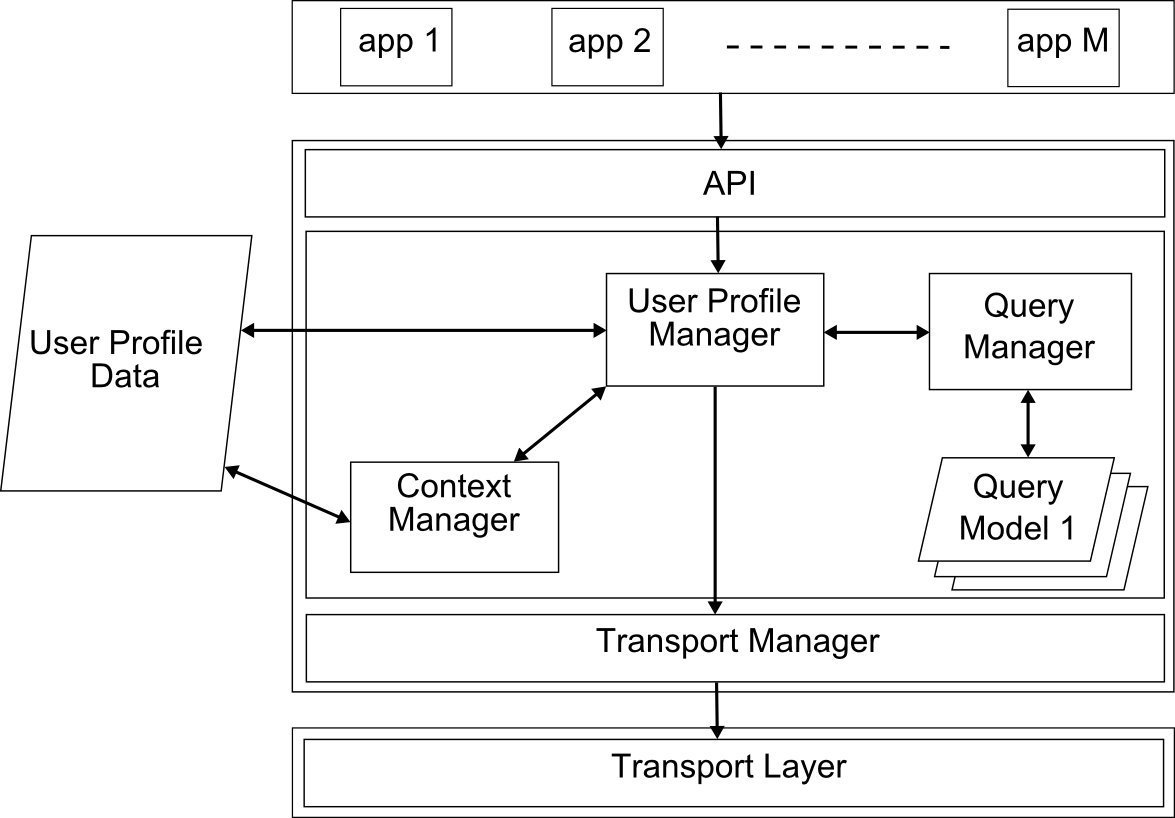
\includegraphics[width=0.5\textwidth]{chellouche1.png}
  \caption{Arquitetura do \emph{middleware} de Chellouche et al\cite{chellouche10}}
  \label{fig:chellouche1}
\end{figure}

\begin{description}
  \item[User profile manager]: módulo central da arquitetura, que interage com todos os outros módulos com o objetivo de construir o perfil correto.
  \item[Context manager]: monitora o ambiente, coletando informações com o objetivo de atualizar a parte dinâmica do perfil.
  \item[Query manager]: módulo responsável por validar e salvar um modelo de consulta para cada aplicação. É construída quando a aplicação é instalada e utilizada quando a aplicação solicita informações.
  \item[Transport manager]: faz a comunicação do perfil de usuário para a aplicação.
  \item[API]: constitui o ponto de interface entre as aplicações e o middleware.
\end{description}

O perfil é construído de acordo com a Figura~\ref{fig:chellouche2}. A aplicação solicita ao gerenciador de perfis, através da API, que por sua vez repassa a solicitação ao gerenciados de consultas. Simultâneo a isto, o gerenciador de contextos é informado que a aplicação está em execução e passa a atualizar o gerenciador de perfis com as informações atualizadas. O perfil de usuário é criado e enviado ao gerenciador de transporte, que retorna o perfil solicitado à aplicação solicitante.

\begin{figure}
  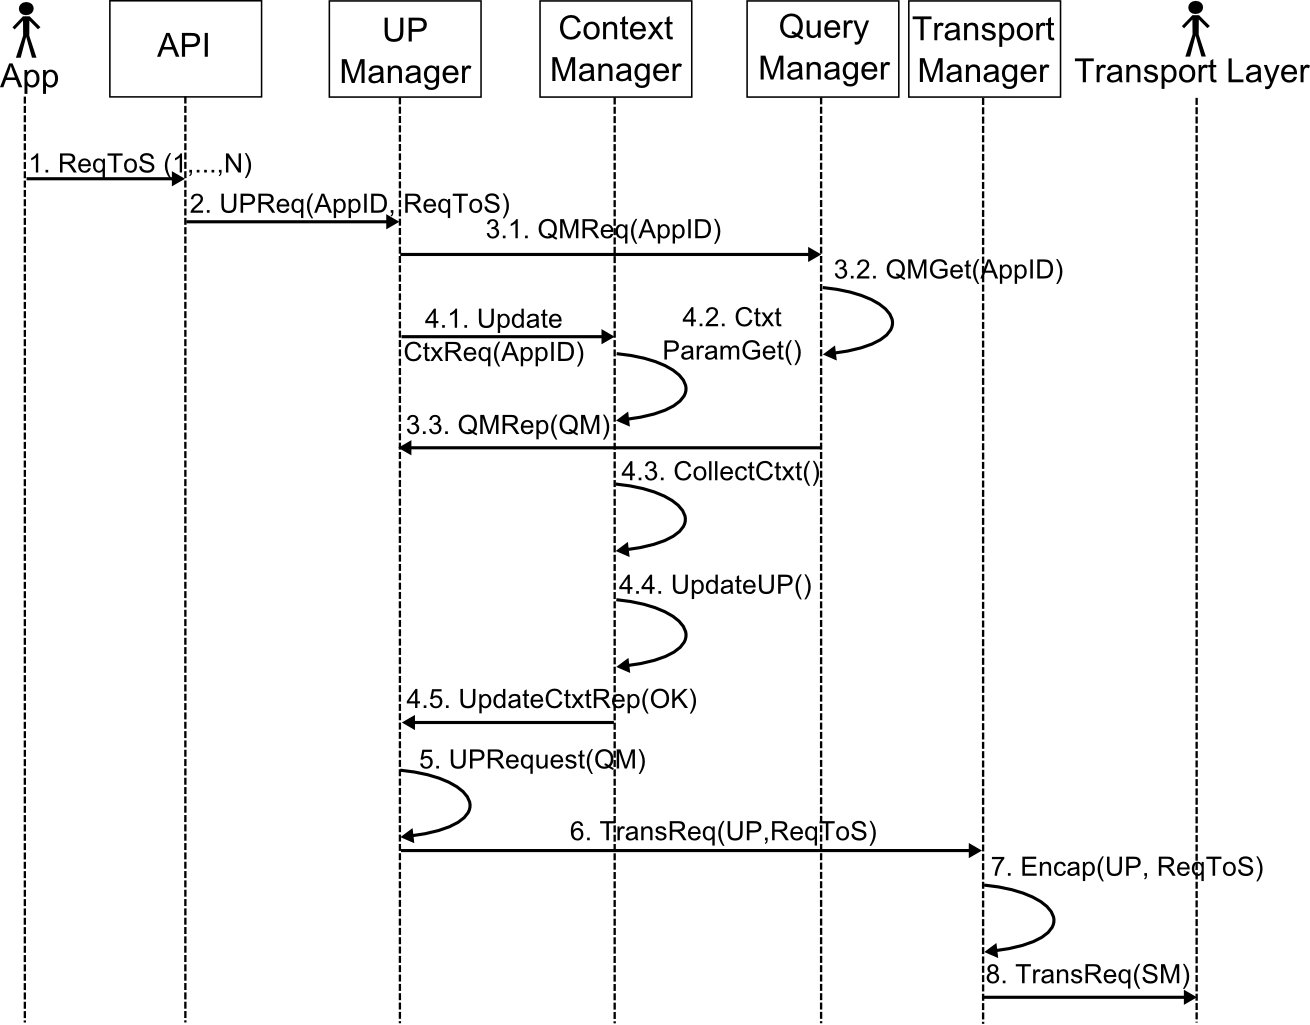
\includegraphics[width=0.5\textwidth]{chellouche2.png}
  \caption{Construção de perfil\cite{chellouche10}}
  \label{fig:chellouche2}
\end{figure}

%%%%%%%%%%%%%%%%%%%%%%%%%%%%%%%%%%%%%%%%%%%%%%%%%%%%%%%%%%%%%%%%%%%%%%%%%%

\subsection{Outros}

\textbf{[Avaliação de outros trabalhos relacionados]}

%%%%%%%%%%%%%%%%%%%%%%%%%%%%%%%%%%%%%%%%%%%%%%%%%%%%%%%%%%%%%%%%%%%%%%%%%%

\subsection{Avaliação dos Ambientes Pesquisados}

A Tabela~\ref{tab:comparacao} exibe um comparativo dos trabalhos apresentados, onde os seguintes fatores são levados em consideração:

\begin{description}
  \item[Interoperável]: se a arquitetura apresentada oferece uma interface que permite operar com outros aplicativos externos, que não aqueles definidos pelo autor;
  \item[Perfis dinâmicos]: se o modelo de perfil permite que os perfis sejam atualizados de acordo com eventos externos, sem a interferência do usuário;
  \item[Campos do perfil]: se o modelo de perfil contém um conjunto pré-definido de campos, ou se as aplicações podem criar novos campos de perfil;
  \item[Armazenamento]: define onde ficam armazenados os perfis do usuário;
  \item[Sensível a contexto]: se o contexto do usuário é levado em consideração na formação do perfil;
  \item[Utiliza trilhas]: se as trilhas do usuário são levadas em consideração na construção do perfil;
  \item[Domínio]: se o perfil é voltado para um domínio específico, ou se o mesmo permite que vários perfis possam ser utilizados.
\end{description}

\begin{table}\centering
  \begin{tabular*}{0.5\textwidth}{@{}lc@{}}
    \toprule
    Característica      & \cite{chellouche10} \\
    \midrule
    Interoperável       & Sim \\
    Perfis Dinâmicos    & Sim \\
    Campos do perfil    & Pré-definido \\
    Armazenamento       & Servidor \\
    Sensível a contexto & Sim \\
    Utiliza trilhas     & Não \\
    Domínio             & Específico \\
    \bottomrule
  \end{tabular*}
  \caption{Comparação entre os trabalhos apresentados}
  \label{tab:comparacao}
\end{table}

%%%%%%%%%%%%%%%%%%%%%%%%%%%%%%%%%%%%%%%%%%%%%%%%%%%%%%%%%%%%%%%%%%%%%%%%%%

\bibliographystyle{ieeetr}

\begin{small}
  \bibliography{../ubicomp}
\end{small}

\end{document}
